\chapter{Testprotokoll Sprint 3}
\section{Test}
\subsection{Angaben zum Test}

\begin{tabularx}{\linewidth}{l l l}
\textbf{datum des Builds} & \textbf{Tester} & \textbf{datum der Testdurchführung}\\
\hline
07.12.15 & Silvan Adrian & 07.12.15

\end{tabularx}

\subsection{Zusammenfassung Ergebnis}
\begin{tabularx}{\linewidth}{l l l}
\textbf{Test durchgeführt?} & \textbf{Tests erfolgreich?} & \textbf{Tests fehlgeschalgen?}\\
\hline
40 (alle) & 40 (alle) & 0 \\
\hline
\end{tabularx}


\subsection{Ergebnisse Tests}
\begin{tabularx}{\linewidth}{X l l}
\textbf{Was} & \textbf{Ok? / nicht OK?} & \textbf{Aufgetretene Fehler}\\
\hline
\textbf{Unit-Tests} & {\color{green} OK}  & keine\\
\hline
Systemtest 1: & & \\
\textbf{Service abonnieren} & {\color{green} OK} & keine\\
\hline
Systemtest 2: & & \\
\textbf{OrderedService kündigen} & {\color{green} OK}  & keine\\
\hline
Systemtest 3: & & \\
\textbf{Abonnierte Services anzeigen} & {\color{green} OK}  & keine\\
\hline
Systemtest 4: & & \\
\textbf{Verfügbare Services anzeigen} & {\color{green} OK}  & keine\\
\hline
Systemtest 5: & & \\
\textbf{ServiceModul bearbeiten} & {\color{green} OK}  & keine\\
\hline
Systemtest 6: & & \\
\textbf{ServiceModul erstellen} & {\color{green} OK}  & keine\\
\hline
Systemtest 6: & & \\
\textbf{ServiceModul löschen} & {\color{green} OK}  & keine\\
\hline
Systemtest 7: & & \\
\textbf{Service bearbeiten} & {\color{green} OK}  & keine\\
\hline
Systemtest 8: & & \\
\textbf{Service erstellen} & {\color{green} OK}  & keine\\
\hline
Systemtest 9: & & \\
\textbf{Service lschen} & {\color{green} OK}  & keine\\
\hline


\end{tabularx}

\newpage

\section{Metriken}
Die abschliessenden Metriken vom Sprint aus SonarQube.
\subsection{Projekt in Zahlen}
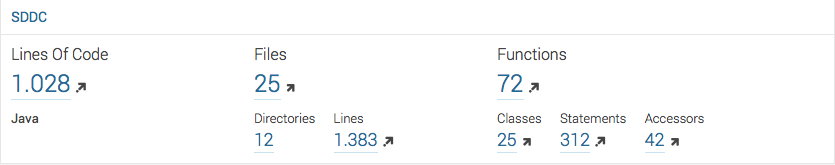
\includegraphics[width=\textwidth]{./10_Protokolle/04_Testprotokoll/images/Sprint3/loc}

\subsection{Unit Tests Coverage}
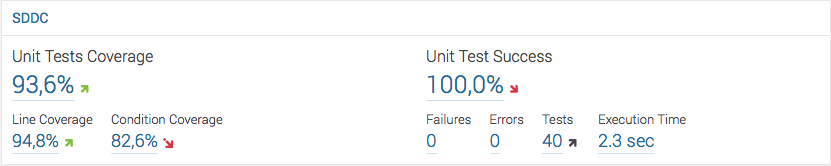
\includegraphics[width=\textwidth]{./10_Protokolle/04_Testprotokoll/images/Sprint3/coverage}

\subsection{Coverage Verteilung auf einzelne Dateien}
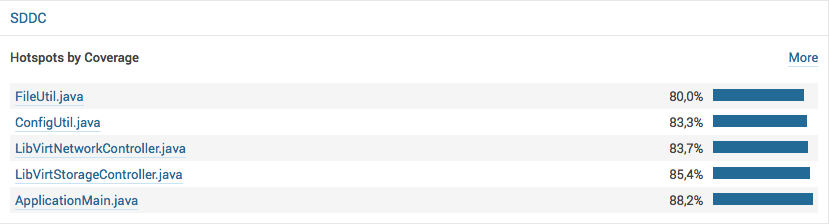
\includegraphics[width=\textwidth]{./10_Protokolle/04_Testprotokoll/images/Sprint3/coverageperfile}

\subsection{Findbugs Issues}
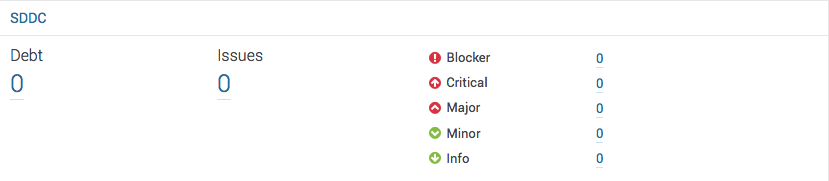
\includegraphics[width=\textwidth]{./10_Protokolle/04_Testprotokoll/images/Sprint3/issues}

\section{Kommentare}

Die Abschliessende App bietet nun ein Admin Dashboard, mit welchem 
Services/Servicemodule
verwaltet werden können und so bestehende Services/Servicemodule gelöscht/bearbeitet oder ganz 
neue Services/Servicemodule erstellt werden.
\newline
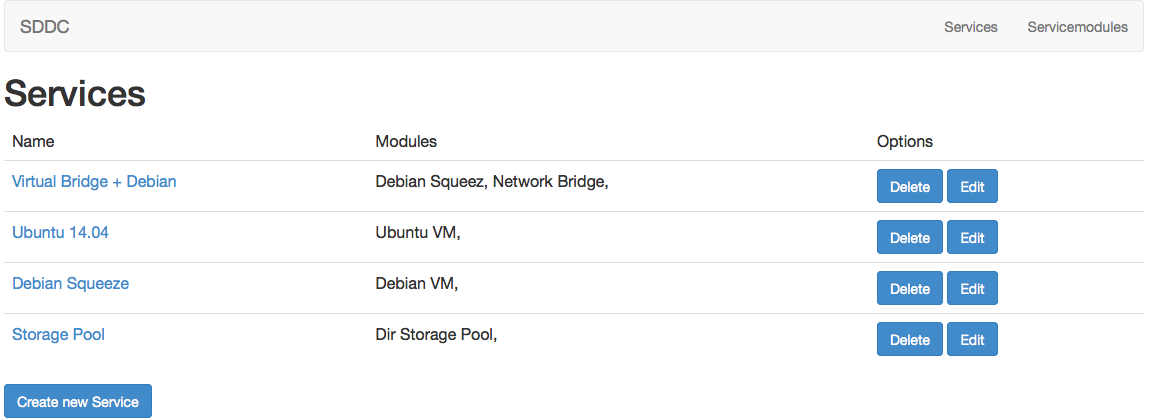
\includegraphics[width=\textwidth]{./10_Protokolle/04_Testprotokoll/images/Sprint3/dashboard}

